\chapter{Transmission lines}\label{lec:lec2}


\begin{mdframed}[backgroundcolor=lightblue, linewidth=1pt, hidealllines=true]
\section{Objectives}
The objectives of this chapter are to discuss the following
\begin{enumerate}[(i)]
\item The concept of voltage and current in high-frequency circuits using a distributed circuit analysis
\item Introduction to Telegrapher's equation and their applications in modelling transmission lines.
\item Definition and derivation of characteristics impedance and reflection coefficient.
\item To find the condition necessary to deliver maximum power to the load i.e. no reflection on the transmission line.
\item To understand the concept of a lossless transmission line.
\item To understand the concept of low-loss transmission lines.
\item To know the test conditions required to determine if a transmission line is a low-loss line.
\item To understand the variation of voltage and current along the transmission line.
\item To understand the concept of Voltage Standing Wave Ratio(VSWR).
\item To know the condition necessary for full reflection at the load end.
\item To know the relationship between the maximum and minimum resistances and VSWR. 
\end{enumerate}
\end{mdframed}

\section{Structures of transmission lines}
Transmission lines are utilized for conveying special cases of electromagnetic waves generated by time-varying voltages and currents. In the previous courses, emphasis was placed on the concept of electromagnetic waves generated by electric and magnetic fields that vary with time.

Transmission lines can best be defined as a medium of power transfer from one point to another. This transmission is done through a variety of structures, some of which are explained below;

\subsection{Co-axial cable}\index{coaxial cable}
\begin{figure}[h]
\centering
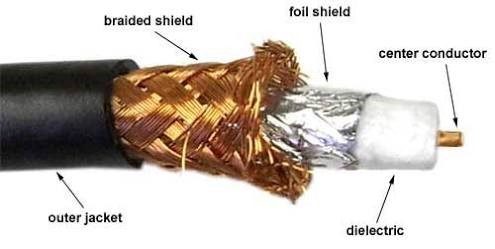
\includegraphics[scale=0.65]{\pathtopartone/graphics/coaxial}
\caption{Co-axial cable transmission line}
\label{fig:coaxial}
\end{figure}

Figure~\ref{fig:coaxial} is a coaxial cable. In this particular setup, there’s an inner and outer conductor and voltage is applied between the inner and outer conductor thus energy will be propagated along the length of the structure.

\subsection{Balanced Parallel wire transmission lines}\index{balanced parallel wire transmission line}
\begin{figure}[h]
\centering
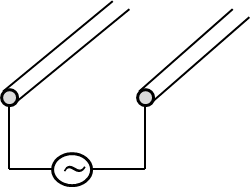
\includegraphics[width=0.5\linewidth]{\pathtopartone/graphics/parallel_wire_tx_simp}
\caption{Balanced parallel wire transmission line}
\label{fig:twowire}
\end{figure}

Figure~\ref{fig:twowire} shows the parallel wire transmission line which has two separate conductors hence when voltage is applied at both ends, energy flows. The voltage on one wire is $V^+$ and the other $V^-$. The voltages are opposite in polarity hence the magnetic field generated by both wires cancels out.

\subsection{Unbalanced Parallel wire transmission lines}\index{unbalanced parallel wire transmission line}
\begin{figure}[h]
\centering
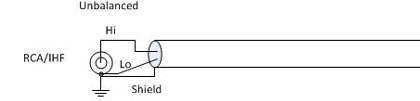
\includegraphics[width=1\linewidth]{\pathtopartone/graphics/unbalanced}
\caption{Unbalanced Line}
\label{fig:unbalanced}
\end{figure}

In this structure shown in Figure~\ref{fig:unbalanced}, we have a conducting rod above a ground surface and voltage is applied between the rod and the ground surface hence power is transmitted efficiently along the structure.

\subsection{Microstrip Line}\index{microstrip line}
\begin{figure}[h]
\centering
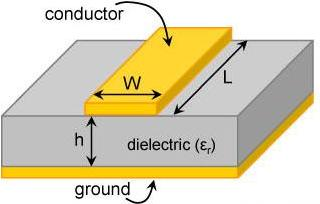
\includegraphics[scale=0.6]{\pathtopartone/graphics/ms (1)}
\caption{Microstrip line}
\label{fig:micro}
\end{figure}

The microstrip line is a transmission line geometry with a single conductor having conducting surfaces at the top and bottom that trace on one side of a dielectric substrate and a single ground plane on the other side (see Figure~\ref{fig:micro}). The single trace is carrying a voltage V with respect to the ground plane. There is no other trace close by carrying the same voltage of opposite polarity to cancel out the magnetic field generated. Hence it is very noisy. The microstrip line is used extensively in printed circuit boards(PCBs).

\subsection{Stripline} 
The structure is made up of a trace of conductor enmeshed in a dielectric with conducting surfaces at the top and bottom that are grounded.(see Figure~\ref{fig:stripline}). The stripline is similar to the microstripline but with ground planes both above and below the trace. Striplines are mostly easily constructed on the inner layers of multi-layer printed circuit boards. Another form of a stripline known as a differential stripline is shown in Figure~\ref{fig:diff-stripline}.
\begin{figure}[h]
\centering
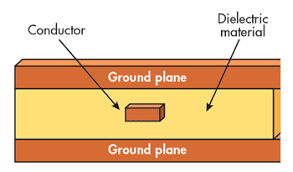
\includegraphics[scale=0.6]{\pathtopartone/graphics/micro}
\caption{Stripline}
\label{fig:stripline}
\end{figure}

\begin{figure}[h]
\centering
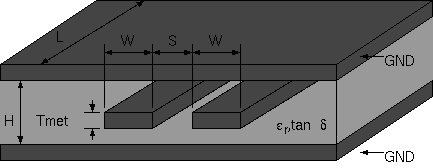
\includegraphics[width=1\linewidth]{\pathtopartone/graphics/stripline}
\caption{Differential Stripline}
\label{fig:diff-stripline}
\end{figure}

\section{Concept of transit time\index{transit time} effect}
A similarity across the various structures is the presence of a two-conductor system, hence when voltage is applied between them because it is a time-varying voltage, current flows through the system. All the structures can be represented by a simple two-conductor system and this is also done for transmission line analysis where we ignore the structure and simply treat it as a two-conductor system, at one end we apply an energy source and at the other end, we apply a load and then carry out analysis from the source to the load.

Circuit laws like Kirchhoff’s law, are limited to low-frequency circuits where we only take note of the value of the electrical components, i.e. for a circuit that comprises circuit elements like resistors, capacitors and inductors, only their values are needed for the circuit analysis. However, as frequency increases, the signal value changes significantly. Let us suppose a transmission line of length, L whose ends are connected to a voltage source and load at points XX'and YY' respectively as shown in Figure~\ref{fig:first}.
\begin{figure}[h]
\centering
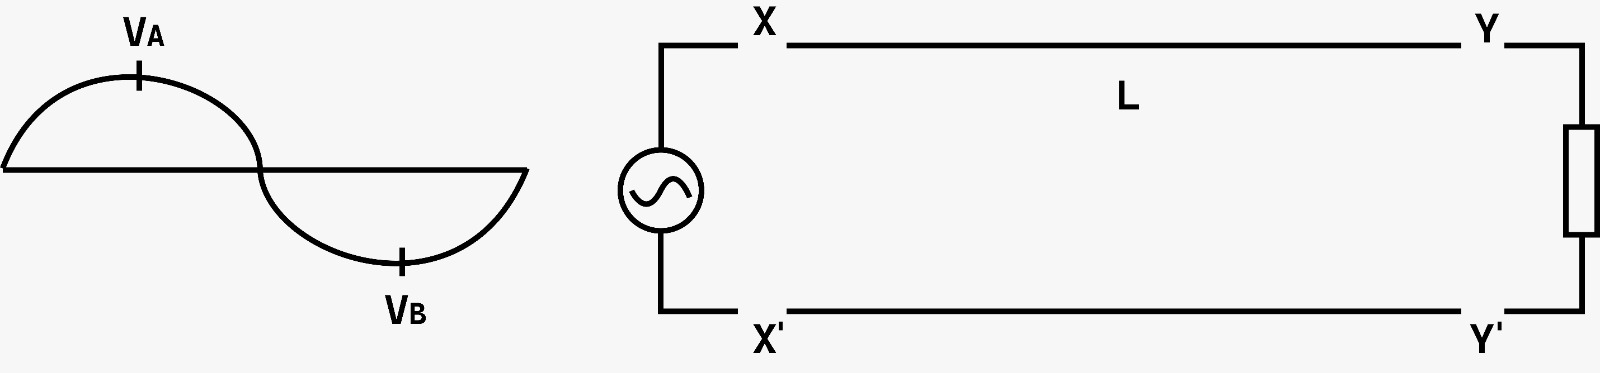
\includegraphics[width=1\linewidth]{\pathtopartone/graphics/fig2.7}
\caption{Circuit diagram of a transmission line}
\label{fig:first}
\end{figure}

At some instant, $ V_{A} $ is applied at X, and when L is sufficiently small relative to the length ($  \lambda = \text{wavelength} $), We assume that $ V_{A} $ appears at Y from X almost instantaneously.

In transit time effect one can realise that $ L \gg\lambda$ and so it is very likely that $ V_{X} \neq V_{Y} $, but when $  \lambda \gg L  $ (for low-frequency circuits) the sinusoidal wave changes almost instantaneously across all points on the line so that we can assume it is constant across the entire length, L. Mathematically, the transit time effect can be expressed in terms of the speed of the transmitted signal, $v$, from point XX' which shows the finite time it takes the voltage at X to appear at Y and it is called \textit{transit time}\index{transit time}.
\begin{align}
t_{r} = \frac{L}{v}
\label{eqn:transittime}
\end{align}

So when a time-varying signal is applied at X, it requires a finite time to travel from X to Y. $ V_{A} $ at X is a time-varying sinusoidal signal such that it takes $ V_{A} $ to appear at Y in transit time, $t_r$. Thus, $ V_{A} $ would have changed to another value say $ V_{B} $, so when a voltage at Y is $ V_{B} $, the voltage at X is $ V_{A} $. In other words, there is a potential difference between X and Y. This difference is related to the length of the cable, the more the length the more the difference, with L very small. $ V_{x} $ is close to $ V_{y} $ as the points A and B will be close to each other and the voltage difference will not be substantial. The important thing here is no matter how small the length we take, there will always be that voltage difference, $ V_{x} – V_{y} \neq 0 $ if $ L > 0 $.

Another observation is that as we increase the frequency, the role of the transit time effect becomes more and more important. So now to the big question; \textit{When do you neglect transit time effect and when do you incorporate it in your design?}

If $ V_{x} – V_{y} $ is small, the transit time effect can be neglected otherwise it should be taken into consideration. Generally, if the transit time is far less than the period of the signal,  $ t_{r} \ll T $ then the transit time effect can be neglected but if $ t_{r} $ is comparable to T, then we have to incorporate the effect of transit time. In other words, when carrying out circuit analysis, the size of the structures starts to play an important role in the analysis.

Recall $T = \frac{1}{f} $, and $t_{r} = \frac{L}{v}$. Given that $ \lambda = \frac{v}{f} $, then $T \gg t_r$ can be expressed as, 
\begin{align*}
\frac{1}{f} \gg \frac{L}{v}\quad\text{or}\quad\lambda \gg L
\end{align*}
Thus, $ \lambda \gg L $ is the condition to neglect the transit time effect.

\section{Concept of Distributed Elements in a transmission line}
With the understanding of \textit{transit time effect}, the transmission of a signal along the transmission line causes a voltage difference across any arbitrary two points on the line. This is contrary to low-frequency circuit analysis (or the \textit{lumped circuit analysis}\index{lumped circuit analysis}), where the circuit idealizes the attributes such as resistance, capacitance and reactance to circuit elements joined by a network of perfecting conducting wires. So how can this observation be modelled? For an ideal conductor, the voltage drop is zero but when the angular frequency, $\omega$ is non-zero, there is a reactive drop and the inductive reactance, $\omega L$ and capacitive susceptance, $\omega C$ becomes significant as frequency increases.

Thus, if an infinitesimal length of the transmission line is assumed to have the lumped element model where the transit time effect is negligible, then a transmission line can be modelled as an aggregation of all the lumped elements. Thus the lumped element is not situated in a particular location but distributed across the entire length of the transmission line. This approach, essentially, will break the \textbf{lumped element} model into a \textbf{distributed element} model. Again, the modelling of each subsection of the transmission line in space is done in such a way that its length is infinitesimally small, $\Delta x$ so that the circuit laws at low frequency can apply within the subsection.


Transit time cannot be neglected for a two-conductor wire but when a small quantity in length is broken down into very Lineal elements of $ \Delta x $ with  $  \Delta x \rightarrow 0 $, The transit time effect can be neglected as $ L \gg \Delta x $ and so the circuit laws of low frequency can be applied to the arbitrary nodes separated by $ \Delta x $ length. In the low-frequency circuit, we should have resistance, capacitance and inductance stated in total value, instead, we have resistance, inductance and capacitance all per unit length.

The relationship between voltage and current is valid for high frequency like that of low frequency as $ \Delta x  \rightarrow 0$ (infinitesimally small). Hence, this solves for voltage and current of a transmission line in the presence of the transit time effect.
\begin{figure}[h]
\centering
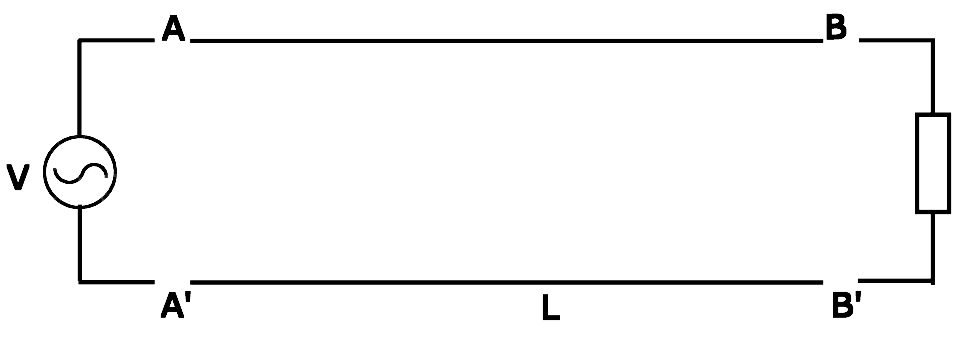
\includegraphics[width=1\linewidth]{\pathtopartone/graphics/second fixed}
\caption{simple circuit diagram of a transmission line}
\end{figure}	

In the circuit above, there is a voltage difference between both ends because of the transit time effect but we do not know why there is a voltage difference.

We all know that as frequency increases in the circuit, the two conductors have both electric and magnetic fields induced as shown below: 

What would be the lumped element model for the subsection of the transmission line? As stated earlier, the voltage drop can be modelled as a resistive and reactive drop across lumped elements. Put differently, We all know that as frequency increases in the circuit, the two conductors XY and X'Y' respectively in Figure~\ref{fig:first} have both electric and magnetic fields induced as shown in Figure~\ref{fig:third}.
\begin{figure}[h]
\centering
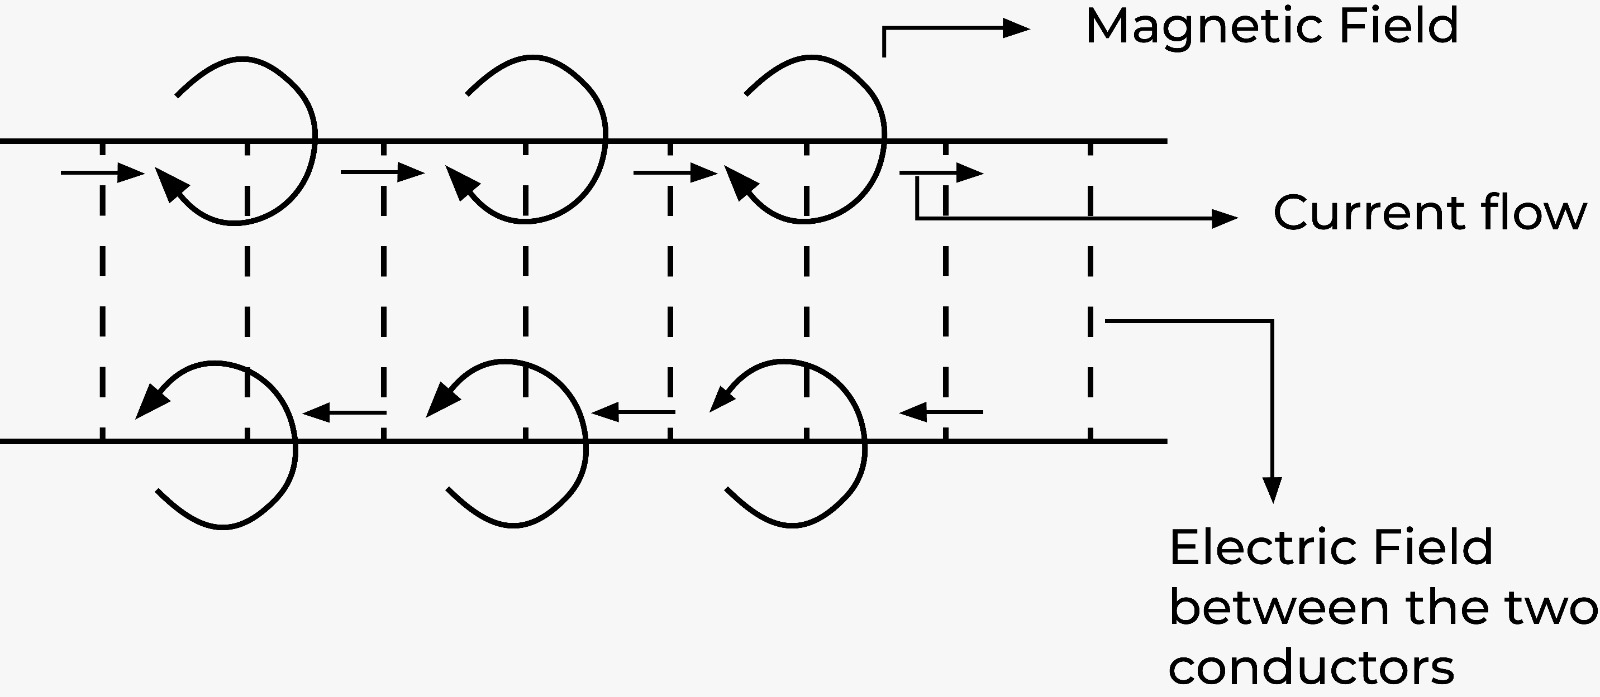
\includegraphics[width=1\linewidth]{\pathtopartone/graphics/fieldsTx}
\caption{Distributed element model explained with generated fields across a transmission line}
\label{fig:third}
\end{figure}

So when the magnetic field is linked with current, an inductance is produced while the electric field between the two conductors with air as dielectric produces capacitance as shown in Figure~\ref{fig:lossless-Tx}. The inductance and capacitance produced are distributed along the length of the structure and these parameters are called the \textbf{distributed parameters of the line}\index{distributed parameters}.
\begin{figure}[h]
\centering
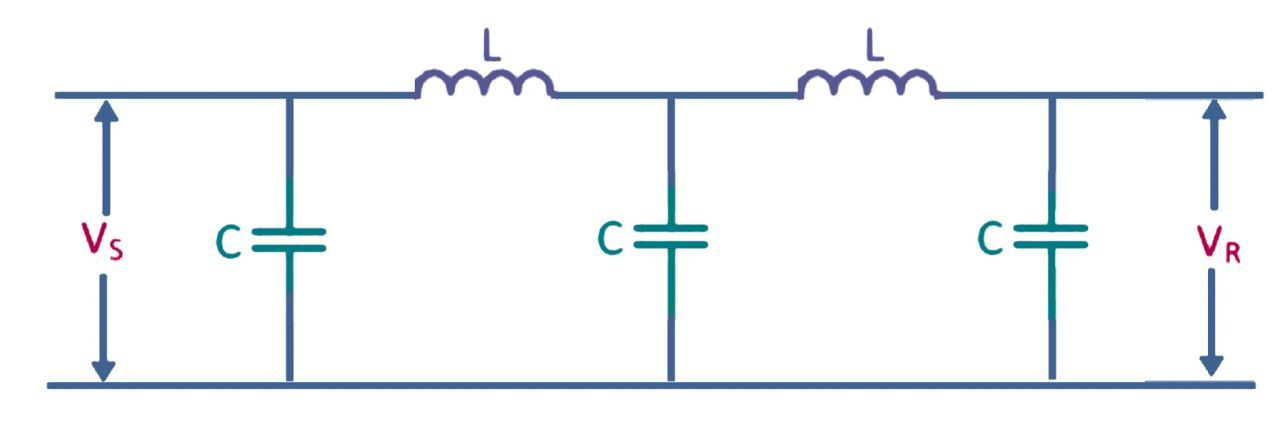
\includegraphics[width=1\linewidth]{\pathtopartone/graphics/transmissionLineLossless}
\caption{Distributed parameters of a lossless transmission line}
\label{fig:lossless-Tx}
\end{figure}

At low frequency, there is no voltage drop across the length of a transmission line but as frequency starts to increase, the inductive reactance, $X_{L}$, starts causing a voltage drop across the length of the transmission line that was not seen at low frequency. Conductors do not have zero resistance and the separation of the conductor, as a dielectric is not ideal, causing current flow between the conductors across the conductance of the dielectric. Hence, we have a more realistic transmission line modelled as shown in Figure~\ref{fig:sixth}
\begin{figure}[h]
\centering
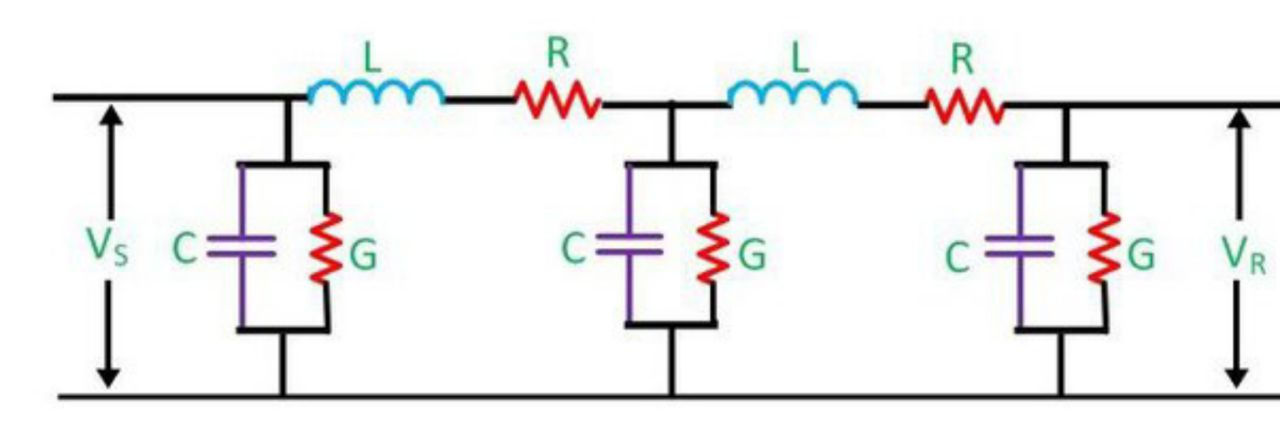
\includegraphics[width=1\linewidth]{\pathtopartone/graphics/transmissionLineLossy}
\caption{Distributed elements for lossy transmission}
\label{fig:transmissionLineLossy}
\end{figure}


From Figure~\ref{fig:sixth}, the resistance, capacitance, inductance and conductance are all per unit length values. We have defined the quantities which are called the \textit{primary constants}\index{primary constants} of the transmission line which are:
\begin{enumerate}[(i)]
\item Resistance per unit length \textemdash\; Ohms/metre
\item Inductance per unit length \textemdash\; Henry/metre
\item Capacitance per metre \textemdash\; Farad/metre
\item Conductance per metre \textemdash\; Siemens/metre
\end{enumerate}
After the primary constants have been determined the analysis of the transmission line can be carried out by:

\begin{enumerate}[(i)]
\item Dividing the transmission line into small segments.
\item Writing down Kirchoff's voltage and current law for the segment.
\item Carrying out the analysis when the segment goes to zero enables the analysis to be valid for any high frequency or any low wavelength. 
\item Applying voltage to the \textbf{lineal segment}\index{lineal segment} that causes current to flow into the circuit.
\end{enumerate}

\section{Telegrapher's Equations}
\begin{figure}[h]
\centering
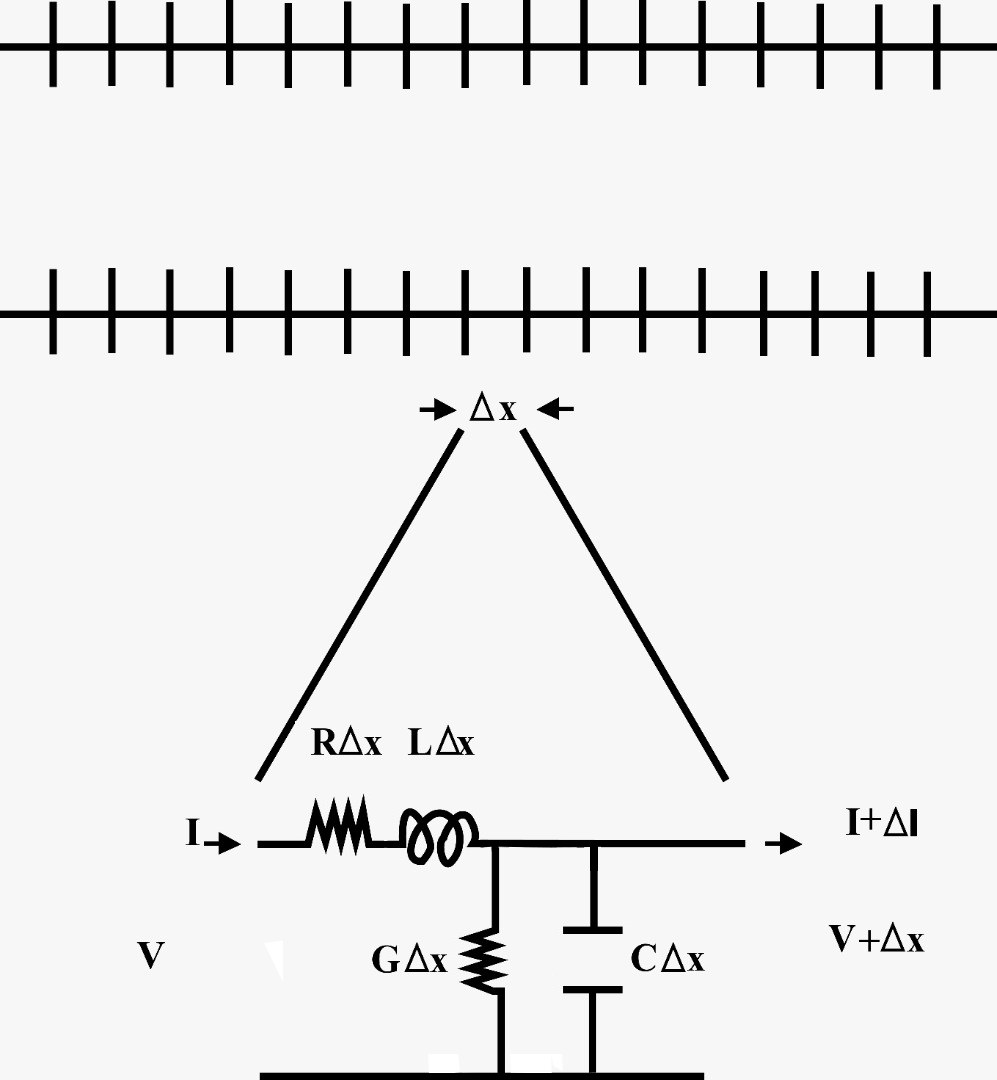
\includegraphics[scale=0.2]{\pathtopartone/graphics/fig 2-11}
\caption{Circuit analysis of a small segment of the transmission line}
\label{fig:seventh}
\end{figure}

Let us now analyse the small segment of the transmission line as shown in Figure~\ref{fig:seventh}. Since the segment is very small and voltage has an angular frequency $ \omega $ the voltage drop and consequent change in current (denoted by $\Delta I$) will be contributed by the resistance and inductance, and conductance and capacitance of the lumped element model. These can be expressed as Equations~\eqref{eqn:voltage} and \eqref{eqn:current}.


\subsection{Let's Understand the Telegrapher's Equations}
First, let's define some terms:
\begin{enumerate}[(i)]
\item \(V_{R}\) is the voltage across resistance
\item \(V_{G}\) is the voltage across conductance
\item \(V_{C}\) is the voltage across capacitance
\item \(V_{L}\) is the voltage across inductance
\end{enumerate}

Now, let's consider each term:
\begin{align*}
&\text{For } V_{R}, \text{ we have } V = IR, \text{ 
\newline
therefore } V_{R} = IR \Delta x.\\
&\text{For } V_{L}, \text{ we have } V_{L} = IX_{L}, \text{ 
\newline therefore } V_{L} = Ij\omega L \Delta x.\\
&\text{For } V_{C}, \text{ we have } V_{C} = I_{C}X_{C}, \text{ 
\newline therefore } V_{C} = \frac{I_{C}}{j\omega C \Delta x}\\
\newline &\text{ hence } I_{C} = V_{C}j\omega C \Delta x.\\
&\text{But } V_{C} = V - \Delta V, \text{ so } I_{C} = (V - \Delta V)(j\omega C \Delta x).\\
&\text{For } V_{G}, \text{ we have } V_{G} = I_{G}R_{G}, \text{ 
\newline therefore } V_{G} = \frac{I_{G}}{G \Delta x}\\
\newline &\text{ hence } I_{G} = V_{G}G \Delta x.\\
&\text{But } V_{G} = V_{C} = V - \Delta V, \text{ so } I_{G} = (V - \Delta V)(G \Delta x).
\end{align*}

Applying Kirchhoff's Voltage Law (KVL) to the small segment of the transmission line, we get
\begin{dmath*}
V - V_{R} - V_{L} - (V - \Delta V) = 0 \text{ implies that $\Delta V = V_{R} + V_{L}$}
\end{dmath*}

Substituting \(V_{R}\) and \(V_{L}\), we get \(\Delta V = IR \Delta x + Ij\omega L \Delta x\).

\begin{dmath*}
V  - IR\Delta x - jI\omega L\Delta x - (V - \Delta V) = 0
\end{dmath*}
Hence,
\begin{align}  
\Delta V = (R \Delta x + j\omega L\Delta x)I
\label{eqn:voltage}
\end{align}

Similarly, applying Kirchoff's current law(KCL), we would have;
\begin{dmath*}
I  - G\Delta x (V - \Delta V) - j\omega C\Delta x (V - \Delta V) - (I - \Delta I) = 0
\end{dmath*}
hence,
\begin{align}
\Delta I = (G \Delta x + j \omega C \Delta x) (V - \Delta V)
\label{eqn:current}
\end{align}

Recall that for Equations~\eqref{eqn:voltage} and \eqref{eqn:current} to be valid at all frequencies, $\Delta x$ must tend to zero.

From Equation~\eqref{eqn:voltage} we have,
\begin{dmath*}
\Delta V =  (R \Delta x + j\omega L\Delta x)I = (R + j\omega L)I\Delta x
\end{dmath*}
\begin{dmath*}
\frac{\Delta V }{\Delta x} = \frac{  (R  + j\omega L)I\Delta x}{\Delta x} =  (R  + j\omega L) I
\end{dmath*}
\[ \lim_{\Delta x\to 0} \frac{\Delta V}{ \Delta x} = \frac{dV}{dx} =  (R + j \omega L)I \]
\begin{align}
\frac{dV}{dx} =  (R + j \omega L)I 
\label{eqn:deltav}
\end{align} 
Also, from Equation~\eqref{eqn:current} we have,
\begin{dmath*}
\Delta I =  (G \Delta x + j\omega C\Delta x) (V - \Delta V) =  (G + j\omega C)(V - \Delta V)
\end{dmath*}
\begin{dmath*}
\frac{\Delta I}{\Delta x} = \frac{  (G + j\omega C)(V - \Delta V)}{\Delta x} =   (G + j\omega C) (V - \Delta V)
\newline
\newline
Substitute, \Delta V 
\newline
\newline
\Delta I = (G\Delta x + j\omega C\Delta x)(V -  (R + j\omega L)I\Delta x)
\end{dmath*}

% \begin{dmath*}

% \Delta I = (G + j\omega C)(V - \Delta V)

% \end{dmath*}

\[ \lim_{ \Delta x\to 0}\frac{ \Delta I}{ \Delta x} = \frac{dI}{dx} =  (G + j\omega C)(V -(R + j\omega L)I\Delta x) \]
\begin{align}
\frac{dI}{dx} = (G + j\omega C)V 
\label{eqn:deltai}
\end{align}
Equations~\eqref{eqn:deltav} and \eqref{eqn:deltai} are said to be coupled equations\index{coupled equations} since $ \frac{dV}{dx} $ is related to $I$ and $ \frac{dI}{dx} $  is related to $V$.

Hence, we see that the voltage and current as $\Delta x \rightarrow 0$ are not related by algebraic equations but by a differential equation. By differentiating Equations~\eqref{eqn:deltav} and \eqref{eqn:deltai} again, we have; 
\begin{align}
\frac{d^{2}V}{dx^{2}} =  (R + j\omega L)\frac{dI}{dx} 
\label{eqn:delta2v}
\end{align}
\begin{align}
\frac{d^{2}I}{dx^{2}} =  (G + j\omega C)\frac{dv}{dx}
\label{eqn:delta2i}
\end{align}

Substituting equation \eqref{eqn:deltai} into \eqref{eqn:delta2v} we have,
\begin{dmath}
\frac{d^{2}V}{dx^{2}} =  (R + j\omega L)\times (G + j\omega C)V = (R + j\omega L)(G + j\omega C)V 
\label{eqn:deqn}
\end{dmath}   
The coefficient of V in Equation~\ref{eqn:deqn} must be a primary quantity of the transmission line since it depends on the primary constant of the transmission line and the frequency of operation $ \omega$. Let's call the quantity $ \gamma^{2}$.

Therefore, 
\begin{align}
\frac{d^{2}V}{dx^{2}} = \gamma^{2}V 
\label{eqn:deqnv}
\end{align}
\begin{align}
\frac{d^{2}I}{dx^{2}} = \gamma^{2}I 
\label{eqn:deqni}
\end{align}
Equations \ref{eqn:deqnv} and \ref{eqn:deqni} are referred to as the \emph{telegrapher's equation}\index{telegraphers equations}.

These are now the voltage and current expressions that govern a transmission line. The quantity $ \gamma $ is called the \emph{propagation constant}\index{propagation constant}. The quantity $V$ and $I$ are sinusoidal and so vary with $e^{j\omega t}$. The quantity $e^{j\omega t}$ helps take care of the harmonic time variation in V and I. 
Since $\gamma$ is a constant for a given line and frequency, 
\[\frac{d^{2}V}{dx^{2}} = \gamma^{2}V\]
Therefore; 
\begin{align}
V(x) = V^{+} e ^{- \gamma x} + V^{-}e^{\gamma x}  
\label{eqn:solnv}
\end{align}
Equation~\eqref{eqn:solnv} is the peak value and $V^+$ and $V^-$ are the arbitrary constants which are evaluated by using appropriate boundary conditions. To find the instantaneous value of $V$, we multiply Equation~\eqref{eqn:solnv} by $e^{j\omega t}$. \footnote{V depends on $x$ and $t$}So,
\begin{dmath}
V(x,t) = V^{+} e^{-\gamma x}e^{j\omega t} + V^{-} e^{\gamma x}e^{j\omega t}
\label{eqn:solnv2}
\end{dmath}
$V(x,t)$ is a complex quantity. The only way to show the amplitude and the initial phase is through a complex number. therefore, $ V^{+}$ is the complex value of voltage at $x=0$ location with a certain initial phase. This is the reason why V is always complex. 

Now, what is the propagation constant, $\gamma$? It is the quantity that defines the characteristics of the signal in the transmission line. It is expressed as $ \gamma = \alpha + j\beta $	 which is also a complex quantity. Substituting $\gamma$ into $V^{+}e^{- \gamma x}e^{j \omega t}$ in Equation~\eqref{eqn:solnv2} gives
\begin{dmath}
V^{+}e^{- \gamma x}e^{j \omega t} = V^{+}e^{-( \alpha + j \beta )x}e^{j \omega t} = V^{+}e^{-\alpha x}e^{j(\omega t - \beta x)}
\end{dmath}

$ V^{+}e^{-\alpha x} $ is a voltage whose amplitude varies exponentially along the transmission line and the phase of the voltage is a combination of space and time i.e. $  (\omega t- \beta x) $, $ \omega t $ for time and $ \beta x  $ for space. Hence $ V^{+}e^{-\gamma x}e^{j\omega t} \equiv V^{+}e^{-\alpha x}e^{j(\omega t-\beta x)} $ is the first point of $V(x,t)$ and represent something whose amplitude varies along the length and the phase of which is a combination of space and time.

For understanding say, $  V^{+} $ is real and positive and $ \alpha= 0 $ then
\begin{align*}
V^{+}e^{-\alpha x}e^{j( \omega t-\beta x)} = V^{+} e^{j( \omega t-\beta x)}
\end{align*}
If we plot this as a function of space and time
\footnote{Recall from Euler's formula; $ e^{j\theta} = cos\theta + jsin\theta $}
\begin{equation*}
V^{+}e^{j( \omega t-\beta x)} = V^{+}cos(\omega t- \beta x) +  V^{+}jsin(\omega t- \beta x)
\end{equation*}
Since we want real voltage we take only $ V^{+}cos(\omega t- \beta x) $ and plot variation of $ V $ with respect to $ x $ and $ t $. We have the graph shown in Figure~\ref{fig:abc} for different $ t $, as $ t $ increases, a point in the plot moves rightward. Hence with respect to space and time, the graph moves rightward as time increases. This is called a \textbf{travelling wave}\index{travelling wave phenomenon}.
\begin{figure}[h]
\centering
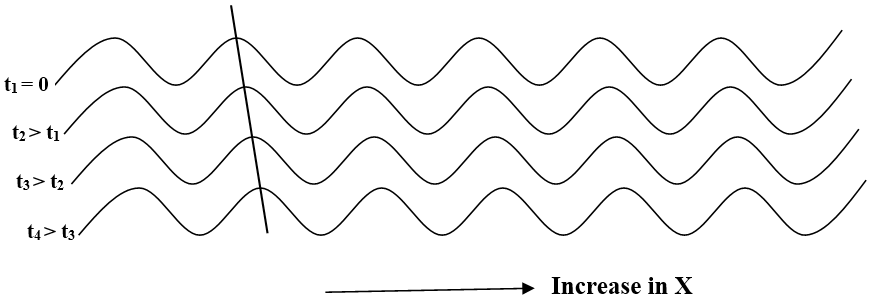
\includegraphics[width=1\linewidth]{\pathtopartone/graphics/ABC}
\caption{Voltage as a function of x for $V^+e^{-\lambda x}$}
\label{fig:abc}
\end{figure}

Hence  $ V^{+}e^{j(\omega t- \beta x )} $ is a positive or progressive travelling wave as it moves rightward with an increase in time. Similarly, when $ V^{-}e^{j( \omega t+ \beta x )} $ is plotted on the graph, the point starts moving leftward with an increase in time and it is the negative travelling wave(see Figure~\ref{fig:abcd}).
\begin{figure}[h]
\centering
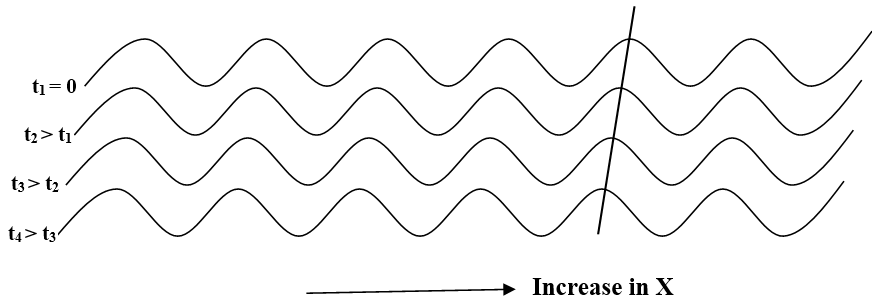
\includegraphics[width=1\linewidth]{\pathtopartone/graphics/ABCD}
\caption{Voltage as a function of x for $V^-e^{+\lambda x}$}
\label{fig:abcd}
\end{figure}

Hence with high-frequency circuit analysis, the voltages and current have to be visualized in the form of waves. In conclusion, we see that a departure from the lumped circuit analysis to the distributed circuit analysis radically changes the approach to circuit analysis to a voltage and current that exist in the form of waves on the electrical circuits. 

\begin{exmp}
\subsubsection*{Transmission line Equation}
Show that the voltage $V(x,t) = A\cos(\omega t+\theta)e^{j\beta x}$ satisfies the transmission line Equation~\eqref{eqn:deqn}, for a uniform lossless line, if $\beta = \omega\sqrt{LC}$.

\subsubsection*{Solution}
In the coming sections, we will discuss the properties of a lossless transmission line in detail but as an introduction, for a lossless transmission line, $R = G = 0$, so Equation~\eqref{eqn:deqn} reduces to
\begin{dmath*}
\derivative[2]{V}{x} = -(0 + j\omega L)\times -(0 + j\omega C)V
= -(\omega^2 LC)V
\end{dmath*}
For $V(x,t) = A\cos(\omega t+\theta)e^{j\beta x}$, the differential equation becomes
\begin{dmath*}
\derivative[2]{A\cos(\omega t+\theta)e^{j\beta x}}{x} = -(\omega^2 LC)\times A\cos(\omega t+\theta)e^{j\beta x}
\end{dmath*}
\begin{dmath*}
A\times -\cos(\omega t+\theta)\times\derivative[2]{e^{j\beta x}}{x} = -(\omega^2 LC)\times A\cos(\omega t+\theta)e^{j\beta x}
\end{dmath*}
\begin{dmath*}
-(A\cos(\omega t+\theta))\times\beta^2e^{j\beta x} = -(\omega^2 LC)\times A\cos(\omega t+\theta)e^{j\beta x}
\end{dmath*}
\begin{dmath*}
\beta^2 = \omega^2 LC
\end{dmath*}

This implies that $\beta = \omega\sqrt{LC}$ and proves that if $\beta = \omega\sqrt{LC}$, the voltage equation given for a lossless transmission line satisfies the transmission line equation.
\end{exmp}


\begin{mdframed}[backgroundcolor=lightblue, linewidth=1pt, hidealllines=true]
\section*{Exercises}
\begin{ExerciseList}
\Exercise[label={ex21}] 
Briefly state and Explain any 5 transmission line structures with appropriate diagrams.

\Exercise[label={ex22}] 
What is the difference between a Stripline and a Microstripline in terms of better noise figures?

\Exercise[label={ex23}] 
With appropriate diagram(s), explain the Transit time effect.

\Exercise[label={ex24}] 
Contrast the lumped element model of a circuit with the distributed element model.

\Exercise[label={ex25}] 
Why are circuit laws for low frequency sufficient for lineal elements created to analyze distributed circuits?

\Exercise[label={ex26}] 
Briefly explain what we mean by the distributed parameters of a transmission line.

\Exercise[label={ex27}] 
$\frac{dV}{dx} = -(R + j\omega L)I$ and  $ \frac{dI}{dx} = -(G + j\omega C)V$ are called coupled equations. Why?

\Exercise[label={ex28}] 
From the first principle and with an appropriate diagram, derive the Telegrapher's equations for a distributed element of a transmission line.

\Exercise[label={ex29}] 
Show that, the general wave equation of a transmission line given as $ V(x,t) = V^{+} e^{-\gamma x}e^{j\omega t} + V^{-} e^{\gamma x}e^{j\omega t} $ is made up of a forward travelling wave and a backward travelling wave.

\Exercise[label={ex210}] 
Write a short note on what we mean by primary constants of a transmission line.

\Exercise[label={ex211}] 
Why is it not practical to use the lumped circuit element model in transmission line problems?

\Exercise[label={ex212}] 
What are the possible sources of losses in a transmission line?

\Exercise[label={ex217}]
From Ex.~\ref{ex212}, show the attenuation constant $\alpha=0$ for a lossless transmission line (i.e. if $R=G=0$).

\Exercise[label={ex217}]
Given the following primary constants and frequency of a transmission line. $R=2\, \text{ohms/m}$, $G=3\, \text{Siemens/m}$, $L=7\, \text{H/m}$, $C=10\, \text{f/m}$ and $freq=40\, \text{MHz}$. Find the propagation constant of the transmission line.
\Answer 2.45 + j2102755994.24

\Exercise[label={ex217}]
Suppose that the propagation constant of a lossless transmission line is $j266572976$. Find the frequency of the transmission line if \text{ohms/m}$, \text{Siemens/m}$, $L=6\, \text{H/m}$ and $C=12\, \text{f/m}$.
\Answer 50GHz 
\end{ExerciseList}
\end{mdframed}
